%\documentclass{beamer}
\documentclass[aspectratio=169]{beamer}
\usepackage{amsmath,amsfonts,amssymb}
\usepackage{beamerthemeshadow}
\usepackage{array}
\usepackage{pgf,pgfarrows,pgfnodes,pgfautomata,pgfheaps,pgfshade}
\usepackage[utf8]{inputenc}
\usepackage{colortbl}
\usepackage{pdfpages}
\usepackage{pythontex}%%Check if we are compiling under latex or pdflatex
% \ifx\pdftexversion\undefined
%   \usepackage[dvips]{graphicx}
%\else
%   \usepackage[pdftex]{graphicx}
%\fi


%\beamertemplatetransparentcovereddynamic
% This is the file main.tex
%\mode<presentation>
{\usetheme{Berlin} }

%% \AtBeginSection[]
%% {
%%    \begin{frame}
%%        \frametitle{Guión}
%%        \tableofcontents[currentsection]
%%    \end{frame}
%% }

\graphicspath{{../figures/}}


\newcommand{\field}[1]{\mathbb{#1}}
\newcommand{\E}{\field{E}}
\newcommand{\R}{\field{R}}
\newcommand{\N}{\field{N}}
\newcommand{\Z}{\field{Z}}
\newcommand{\Q}{\field{Q}}
\newcommand{\EE}{\field{E}}
\newcommand{\FF}{\field{F}}
\newcommand{\GG}{\field{G}}
\renewcommand{\L}{\field{L}}
\renewcommand{\P}{\field{P}}
\newcommand{\LL}{{\mathfrak L}}

\renewcommand{\arraystretch}{1.5}
\hypersetup{
   pdfpagemode={FullScreen},
   pdftitle = {},
   pdfauthor={Mathieu Kessler},
colorlinks=true,linkcolor=red
}

\title{Regresión simple, múltiple, y clasificación (1)}
\author[Kessler]{Mathieu Kessler}
\institute[UPCT]{
  Departamento de Matemática Aplicada y Estadística\\
  Universidad Politécnica de Cartagena}

\date[Cartagena]{Cartagena}

\begin{document}

\begin{frame}
  \titlepage
\end{frame}
 \begin{frame}
   \begin{block}{Conjuntos de datos reales}
     \begin{itemize}
     \item<+-> A menudo, un individuo está descrito por una serie de características (en inglés ``features''), o variables.
     \item<+-> En base a los valores de estas características, podemos estar interesados en:
       \begin{enumerate}
       \item Clasificar cada individuo en una determinada categoría.
       \item Predecir el valor de una cantidad de interés $y$ para un individuo.
       \end{enumerate}
     \end{itemize}
   \end{block}
 \end{frame}
\begin{frame}\frametitle{Ejemplo: problema de clasificación}
  {\scriptsize \begin{itemize}
  \item<+-> Queremos reconocer de manera automática los códigos postales escritos a mano en sobres
  \item<+-> Aislamos imágenes 20x20 píxeles de cada dígito en el código postal:
  \begin{center}
    \includegraphics[height=4cm]{digito-09.png}
  \end{center}
\item<+-> Las características son $x_1$, $x_2$, $\ldots$ $x_{400}$, la intensidad de gris en cada pixel.
\item<+-> Basándonos en esas características, queremos clasificar el dígito en una de las categorías ``0'', ``1'', ``2'', $\ldots$, ``9''.
  \end{itemize}
}
 \end{frame}

\begin{frame}\frametitle{Ejemplo: problema de predicción}
 \begin{itemize}
  \item<+-> Queremos predecir la demanda de energía eléctrica de un conjunto de clientes con un día de antelación.
  \item<+-> Las características que consideramos pueden incluir: temperatura ambiente, ¿es día festivo?, contexto económico, ¿hay huelga?  
\item<+-> Basándonos en esas características para el día siguiente, queremos obtener una predicción de $y$, la demanda electríca para mañana.
  \end{itemize}
 \end{frame}

 \begin{frame}{Planteamiento}
Tenemos un conjunto de datos del que podemos aprender:\\
Para un cierto número de individuos,
\onslide<2->
\begin{itemize}
\item Por una parte, hemos observado sus características $$x_1,x_2,\ldots, x_k.$$
\item<3-> Pero también hemos observado:
  \begin{itemize}
  \item<4->   para el problema de clasificación, a qué categoría pertenece. Se recoge en una variable $y$ que toma valores discretos (las categorías). 
  \item<5-> para el problema de predicción, el valor que toma la variable de interés $y$ para cada uno de esos individuos.
  \end{itemize}
\end{itemize}
\onslide<6-> 
\begin{center}
  \fbox{\textcolor{red}{``Learning set''}}
\end{center}
 \end{frame}
 \begin{frame}\frametitle{Planteamiento}
   \begin{itemize}
   \item Usaremos un algoritmo  (``learning algorithm''), que aprenda del conjunto de aprendizaje, de manera que, para un nuevo individuo, con características $x_1,\ldots,x_k$ (que no tengan por qué corresponder exactamente con valores ya observados en el conjunto de aprendizaje), nos proporcione una predicción del valor de $y$.
   \end{itemize}
   
 \end{frame}

 \begin{frame}
   \begin{block}{Empezamos por ilustrar los conceptos con el problema de predicción}
Consideraremos 
     \begin{itemize}
     \item Una variable $y$ (también llamada \alert{respuesta})
     \item $k$ variables o  \alert{características}  $x_1, x_2, \ldots, x_k$.
     \end{itemize}
\onslide<2->
Buscamos aprender para predecir el valor de $y$  en función del valor
observado de  $x_1, x_2, \ldots, x_k$.
   \end{block}

 \end{frame}
       \begin{frame}{Ejemplos de conjuntos de datos reales}
% {\scriptsize Resistencia del cemento en función del tiempo de fraguado en días (Hald 1952)}
% \vspace{-1cm}\begin{center}
%     \includegraphics[height=7cm]{cemento}
%   \end{center}
   
%  \end{frame}
%  \begin{frame}{Ejemplos de cuatro conjuntos de datos reales}
{\scriptsize Nivel máximo anual del mar en Venecia}
\begin{center}
    \includegraphics[height=6cm]{venecia.png}
  \end{center}
   
 \end{frame}
%  \begin{frame}{Ejemplos de cuatro conjuntos de datos reales}
% {\scriptsize Producción mundial de petróleo}
% \vspace{-1cm}\begin{center}
%     \includegraphics[height=7cm]{petroleo}
%   \end{center}
   
%  \end{frame}
 \begin{frame}{Ejemplos de conjuntos de datos reales}
{\scriptsize Velocidad de Recesión de 24 nebulosas}
\vspace{-1cm}\begin{center}
    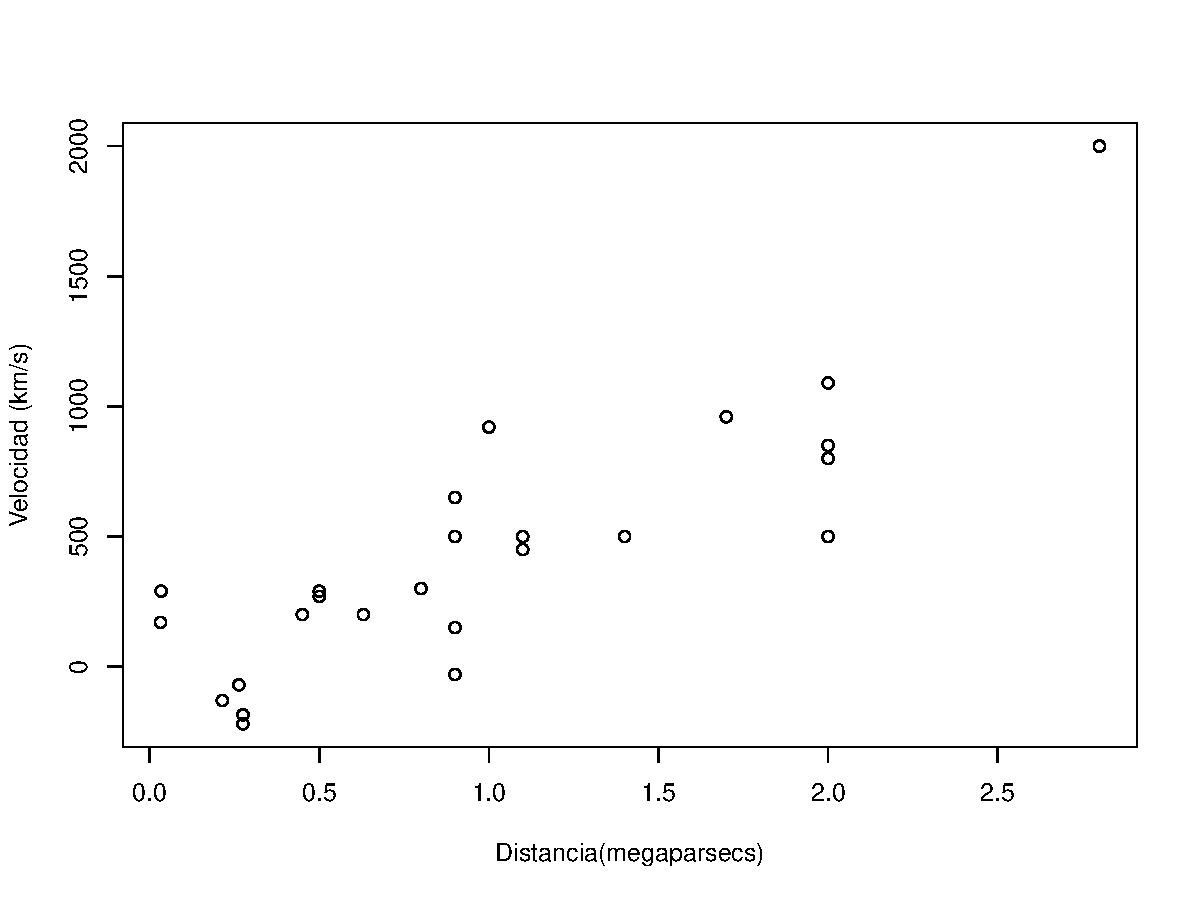
\includegraphics[height=7cm]{hubble}
  \end{center}
   
 \end{frame}
 \begin{frame}{Ejemplos de conjuntos de datos reales}
{\scriptsize Superficie de respuesta}
\vspace{-1cm}\begin{center}
  \includegraphics[height=6cm]{response_surface}

  {\tiny Fuente:
     https://commons.wikimedia.org/wiki/File:Estimated\_response\_surface3.png
  Attribution: Cjp24, CC BY-SA 3.0, via Wikimedia
  Commons.
  }
  \end{center}
   
\end{frame}

\begin{frame}{Ejemplos de conjuntos de datos reales}
{\scriptsize Rendimiento de una reacción}
\vspace{-1cm}\begin{center}
    \includegraphics[height=6cm]{yield_heatmap}
  \end{center}\vspace{-0.5cm}

   {\tiny Fuente: http://www.wright.edu/~oleg.paliy/Papers/PCR\_modeling/FigureS5.png}


 \end{frame}

 \begin{frame}

   \begin{block}{Los datos}

      Nuestro conjunto de aprendizaje:\\
       \begin{center}
\begin{tabular}{lllll}
$Y$&$X_1$&$X_2$&$\cdots$&$X_k$\\ \hline
$y_1$&$x_{11}$&$x_{12}$&$\cdots$&$x_{1k}$\\
\vdots&\vdots&\vdots&\vdots&\vdots\\
$y_{n}$&$x_{n1}$&$x_{n2}$&$\cdots$&$x_{nk}$\\
\end{tabular}
\end{center}
Cada fila representa un individuo, cada columna una variable o característica para ese individuo.\\
\onslide<2-> Usaremos la notación $$x_{i\bullet}=(x_{i0},x_{i1},\dots,x_{ik})^T$$ para denotar el vector de características del individuo número $i$ \textit{(hemos incluido $x_{i0}=1$.)}

   \end{block}
 \end{frame}
 \begin{frame}{Nuestro conjunto de aprendizaje, con sólo una
     característica $x$.}
\vspace{-0.5cm}
\begin{center}
    \includegraphics[height=7cm]{nube.png}
     \end{center}   
 \end{frame}
 \begin{frame}
   \begin{block}{Decidimos explicar la relación entre $x_1, x_2,
       \ldots, x_k$ e $y$ usando una determinada forma funcional}
     \begin{itemize}
     \item<+-> Por ejemplo, con una característica,  una recta: $y=ax_1+b$.
     \item<+-> Por ejemplo, con dos características, un parabolóide:
       $y=a_{00}+a_{10}x_1+a_{01}x_2+a_{20}x_1^2+a_{02}x_2^2+a_{11}x_1x_2$.
     \item<+-> En general, especificamos una familia paramétrica:
$$y=f(\theta,x_0, x_1, \ldots, x_k)\quad \theta=(\theta_0, \theta_1,\ldots,\theta_k),$$
$\theta$ es un vector de parámetros.
     \end{itemize}
\onslide<4-> A veces llamamos a la relación $y=f(\theta,x_0,x_1,
\ldots, x_k)$ la ``hipótesis''.    
   \end{block}\onslide<5->
   \begin{block}{Nuestro objetivo: aprender del conjunto de aprendizaje,}
 es decir determinar  la función de la familia que proporcione la \alert{mejor} adecuación al conjunto de aprendizaje \onslide<5-> $\Leftrightarrow$ Debemos aprender el valor concreto de $\theta$ que corresponde a esa función óptima.
   \end{block}
 \end{frame}

 \begin{frame}{Nuestro concepto de ``mejor'': la función coste}
   \begin{block}{Introducimos una función de coste}
     \begin{itemize}
     \item<+-> Asocia para un valor concreto de $\theta$ un valor númerico que refleje la calidad del ajuste de nuestra funcional o hipótesis al conjunto de aprendizaje.
     \item<+-> Es una función que denotamos por $$\theta\mapsto J(\theta).$$
     \end{itemize}
   \end{block}
\onslide<3->
   \begin{block}{Nuestro objetivo será: }
Encontrar el valor de $\theta$ que minimiza el coste, es decir tendremos que resolver el problema de miminización:\vspace{-0.3cm}
$$\min_{\theta}J(\theta).$$
     
   \end{block}
 \end{frame}
\begin{frame}{La función de coste que consideraremos}
   \begin{block}{}
    {\scriptsize Buscamos que sean mínimas las distancias entre los
      valores de $y$ observados en el conjunto de aprendizaje, es
      decir $y_1,\ y_2,\ldots y_n$,  y sus valores predichos por la
      hipótesis: $f(\theta,x_{10},x_{11},\ldots, x_{1k})$,
      $f(\theta,x_{20},x_{21},\ldots, x_{2k})$, $\ldots$, $\ f(\theta,x_{n0},x_{n1},\ldots, x_{nk})$.}
   \end{block}
    \includegraphics[height=6cm]{nubeajuste.png}
  \end{frame}

\begin{frame}{La función de coste}
\begin{overlayarea}{\textwidth}{4cm}
Definimos la función de coste: 
%$$J(\theta)=(\only<2>{\alertQ{y_1}}\only<1,3->{y_1}-f(\only<3>{\alert{\theta}}\only<1-2,4->{\theta},\only<2>{\alert{x_1}}\only<1,3->{x_1}))^2+\cdots+(\only<2>{\alert{y_n}}\only<1,3->{y_n}-f(\only<3>{\alert{\theta}}\only<1-2,4->{\theta},\only<2>{\alert{x_n}}\only<1,3->{x_n}))^2.$$
$$J(\textcolor{red}{\theta})=\frac 1 n \left[(\textcolor{green}{y_1}-f(\textcolor{red}{\theta},\textcolor{green}{x_{10},\ldots,x_{1k}}))^2+\cdots+(\textcolor{green}{y_n}-f(\textcolor{red}{\theta},\textcolor{green}{x_{n0},\ldots,x_{nk}}))^2\right].$$
Buscamos el valor $\hat\theta$ de $\theta$ que minimiza $\theta\mapsto J(\theta)$.
\onslide<2->
\begin{block}{Nota}
  \begin{itemize}
  \item   En $J(\theta)$, \textcolor{green}{$x_{10},\ldots,x_{nk}$} e
    \textcolor{green}{$y_1,\ldots,y_n$} son valores fijados concretos
    (conjunto de aprendizaje).  Sólo \alert{$\theta$} es variable:
    $\theta\mapsto J(\theta)$ es una función de $\theta$.
  \item \textcolor{red}{$\theta$} es un vector.
  \end{itemize}
\end{block}
\end{overlayarea}
\end{frame}

\begin{frame}{Un primer ejemplo}
Nuestro conjunto de aprendizaje:
\begin{center}
  \includegraphics[height=4.5cm]{rectaorigen.png}
\end{center}
  \onslide<2-> Nuestra hipótesis: $$f(\theta,x_1)=\theta_1x_1,$$
es decir, una recta forzada por el origen.
\end{frame}

\begin{frame}{La función de coste}
  \begin{overlayarea}{\textwidth}{\textheight}
    Tenemos un único parámetro $\theta=\theta_1$, podemos representar
    la función de coste.\\
    \vphantom{Con su mínimo}
    \begin{center}
      
  \includegraphics[height=4.5cm]{funcionccosterectaorigen.png}
\end{center}
\end{overlayarea}
\end{frame}
\begin{frame}{La función de coste}
    \begin{overlayarea}{\textwidth}{\textheight}
Tenemos un único parámetro $\theta=\theta_1$, podemos representar la
función de coste.\\
Con su mínimo:
\begin{center}
  \includegraphics[height=4.5cm]{funcionccosterectaorigen_con_min.png}
\end{center}
\end{overlayarea}
\end{frame}

\begin{frame}{Un segundo ejemplo}
Mismo  conjunto de aprendizaje:
\begin{center}
  \includegraphics[height=4.5cm]{rectaorigen.png}
\end{center}
  \onslide<2-> Nuestra hipótesis: $$f(\theta,x_1)=\theta_0+\theta_1x_1,$$
es decir, ahora admitimos una ordenada al origen
\end{frame}
\begin{frame}{La función de coste}
  Tenemos dos parámetros:  representamos la función de coste como una
  superficie: 
\begin{center}
  \includegraphics[height=6cm]{superficie_funcion_coste.png}
\end{center}  
\end{frame}

\begin{frame}{La función de coste}
  O usando curvas de nivel:
\begin{center}
  \includegraphics[height=6cm]{contour_coste_recta.png}
\end{center}
\end{frame}
\begin{frame}{La función de coste}
  Situamos el mínimo:
\begin{center}
  \includegraphics[height=6cm]{contour_coste_recta_con_min.png}
\end{center}
\end{frame}
\begin{frame}{Procedimiento numérico de minimización: el algoritmo del
    gradiente (``gradient descent'')}
\begin{block}{Idea básica}
  \begin{itemize}
\item<+-> Queremos minimizar una función  $(\theta_0,\ldots, \theta_k)\mapsto J(\theta_0,\ldots\theta_k)$, es decir encontrar $\theta$ situado en el mínimo de la superficie \textit{\scriptsize(en un espacio de $k+2$ dimensiones)}
\item<+-> El  procedimiento consistirá en:
\begin{description}
\item[\textcolor{red}{Inicializar:}]<+-> empezamos con un vector $(\theta_0,\ldots \theta_k)$ inicial.
\item[\textcolor{red}{Iterar:}]<+-> modificamos el vector $(\theta_0,\ldots\theta_k)$ para disminuir el valor del coste.
\item[\textcolor{red}{Parar:}]<+-> decidimos de un cierto criterio de parada.
\end{description}
\end{itemize}
\end{block}

\end{frame}

\begin{frame}{``Gradient descent''}

  {\scriptsize (Imagen de Andrew Ng, Stanford:)}
\begin{center}
  \includegraphics[height=6cm]{gradient-descent-ng.png}
\end{center}
\end{frame}
\begin{frame}
\frametitle{Algoritmo de ``Gradient descent''.}
\begin{itemize}
\item<2-> Partimos de un vector inicial $(\theta_0,\theta_1, \ldots, \theta_k)$.
\item<3-> La actualización de $\theta = (\theta_0,\theta_1,
  \ldots,\theta_k)$ en cada iteración (``valor actual de $\theta$'') aprovecha el gradiente de la función coste:
$$\left\{\begin{array}{lcl}
\theta_0&\leftarrow &\theta_0-\alpha\frac{\partial}{\partial \theta_0}J(\theta),\\
\theta_1&\leftarrow &\theta_1-\alpha\frac{\partial}{\partial \theta_1}J(\theta),\\
\vdots&\vdots&\vdots\\
\theta_k&\leftarrow &\theta_k-\alpha\frac{\partial}{\partial \theta_k}J(\theta),\\
\end{array}\right.$$
donde $\alpha$ es la tasa de aprendizaje (``learning rate''), un parámetro positivo que fijamos.
\end{itemize}
\onslide<4->
\begin{block}{Nota}
{\scriptsize La actualización en cada iteración se hace de manera
  simultánea para todos los componentes de $\theta$, es decir que el
  gradiente es evaluado en el mismo vector
  $(\theta_0,\theta_1,\ldots,\theta_k)$ en todas las líneas.} 
  
\end{block}
\end{frame}

\begin{frame}\frametitle{El algoritmo del gradiente}
La modificación se hace de manera simultánea, es decir,
$$\left\{\begin{array}{lcl}
\textcolor{red}{\theta_0}&\leftarrow &\textcolor{green}{\theta_0}-\alpha\frac{\partial}{\partial \theta_0}J(\textcolor{green}{\theta}),\\
\textcolor{red}{\theta_1}&\leftarrow &\textcolor{green}{\theta_1}-\alpha\frac{\partial}{\partial \theta_1}J(\textcolor{green}{\theta}),\\
\vdots&\vdots&\vdots\\
\textcolor{red}{\theta_k}&\leftarrow &\textcolor{green}{\theta_k}-\alpha\frac{\partial}{\partial \theta_k}J(\textcolor{green}{\theta}),\\
\end{array}\right.$$

\begin{itemize}
\item En \textcolor{green}{verde}: el valor de $\theta$ proviniente de la etapa anterior
\item  En \textcolor{red}{rojo}: el valor de $\theta$ actualizado en la etapa actual.
\end{itemize}

\end{frame}

\begin{frame}
\frametitle{Algoritmo de ``Gradient descent''.}
\begin{itemize}
\item Partimos de un vector $(\theta_0,\theta_1,\ldots,\theta_k)$.
\item<+-> La actualización de $(\theta_0,\theta_1,\ldots,\theta_k)$ en cada iteración aprovecha el gradiente de la función coste:
$$\left\{\begin{array}{lcl}
           \left(\begin{array}{c}\theta_0\\
                   \vdots\\
  \theta_k
\end{array}
           \right)&\leftarrow& \left(\begin{array}{c}\theta_0\\
                                       \vdots\\
\theta_1
\end{array}
\right)-\alpha\,\nabla J(\theta),\\
\end{array}\right.$$
donde $\alpha$ es la tasa de aprendizaje (``learning rate''), un parámetro positivo que fijamos.
\end{itemize}
\begin{block}{Nota}
{\scriptsize La actualización en cada iteración se hace de manera
  simultánea para $\theta_0, \ldots,\theta_k$, es decir que el gradiente es evaluado en el mismo vector $\theta$ en ambas líneas.} 
  
\end{block}
\end{frame}
\begin{frame}
 \frametitle{Intuición para el algoritmo}
 \begin{overlayarea}{\textwidth}{8cm}
 Es más fácil verlo si tenemos sólo un parámetro $\theta_1\mapsto J(\theta_1)$.
\begin{center}
  \includegraphics[height=4.5cm]{funcionccosterectaorigen.png}
\end{center}
%Si parto de un punto a la derecha, la pendiente (gradiente) es positiva, por lo que el paso reduce el valor de $\theta_1$.   
 \end{overlayarea}
\end{frame}
\begin{frame}
 \frametitle{Intuición para el algoritmo}
 \begin{overlayarea}{\textwidth}{8cm}
 Es más fácil verlo si tenemos sólo un parámetro $\theta_1\mapsto J(\theta_1)$.
\begin{center}
  \includegraphics[height=4.5cm]{gradientdescent-derecha-1.png}
\end{center}
Si parto de un punto a la derecha, la pendiente (gradiente) es positiva, \vphantom{por lo que el paso reduce el valor de $\theta_1$.}   
 \end{overlayarea}
\end{frame}

\begin{frame}
 \frametitle{Intuición para el algoritmo}
 \begin{overlayarea}{\textwidth}{8cm}
 Es más fácil verlo si tenemos sólo un parámetro $\theta_1\mapsto J(\theta_1)$.
\begin{center}
  \includegraphics[height=4.5cm]{gradientdescent-derecha-2.png}
\end{center}
Si parto de un punto a la derecha, la pendiente (gradiente) es positiva, por lo que el paso \textcolor{red}{reduce} el valor de $\theta_1$.   
 \end{overlayarea}
\end{frame}
\begin{frame}
 \frametitle{Intuición para el algoritmo}
 \begin{overlayarea}{\textwidth}{8cm}
 Es más fácil verlo si tenemos sólo un parámetro $\theta_1\mapsto J(\theta_1)$.
\begin{center}
  \includegraphics[height=4.5cm]{gradientdescent-izquierda-1.png}
\end{center}
Si parto de un punto a la izquierda, la pendiente (gradiente) es negativa, \vphantom{por lo que el paso aumenta el valor de $\theta_1$.}   
 \end{overlayarea}
\end{frame}

\begin{frame}
 \frametitle{Intuición para el algoritmo}
 \begin{overlayarea}{\textwidth}{8cm}
 Es más fácil verlo si tenemos sólo un parámetro $\theta_1\mapsto J(\theta_1)$.
\begin{center}
  \includegraphics[height=4.5cm]{gradientdescent-izquierda-2.png}
\end{center}
Si parto de un punto a la izquierda, la pendiente (gradiente) es negativa, por lo que el paso \textcolor{red}{aumenta} el valor de $\theta_1$.   
 \end{overlayarea}
\end{frame}


\begin{frame}
 \frametitle{Intuición para el algoritmo}
 \begin{overlayarea}{\textwidth}{8cm}
Es importante la elección de $\alpha$. Si $\alpha$ es demasiado pequeño, el algoritmo converge muy lentamente,
\begin{center}
  \includegraphics[height=4.5cm]{gradientdescent-smallalpha-1.png}
\end{center}
 \end{overlayarea}
\end{frame}

\begin{frame}
 \frametitle{Intuición para el algoritmo}
 \begin{overlayarea}{\textwidth}{8cm}
Es importante la elección de $\alpha$. Si $\alpha$ es demasiado pequeño, el algoritmo converge muy lentamente,
\begin{center}
  \includegraphics[height=4.5cm]{gradientdescent-smallalpha-2.png}
\end{center}
 \end{overlayarea}
\end{frame}

\begin{frame}
 \frametitle{Intuición para el algoritmo}
 \begin{overlayarea}{\textwidth}{8cm}
Es importante la elección de $\alpha$. Si $\alpha$ es demasiado pequeño, el algoritmo converge muy lentamente,
\begin{center}
  \includegraphics[height=4.5cm]{gradientdescent-smallalpha-3.png}
\end{center}
 \end{overlayarea}
\end{frame}

\begin{frame}
 \frametitle{Intuición para el algoritmo}
 \begin{overlayarea}{\textwidth}{8cm}
Es importante la elección de $\alpha$. Si $\alpha$ es demasiado pequeño, el algoritmo converge muy lentamente,
\begin{center}
  \includegraphics[height=4.5cm]{gradientdescent-smallalpha-4.png}
\end{center}
 \end{overlayarea}
\end{frame}

\begin{frame}
 \frametitle{Intuición para el algoritmo}
 \begin{overlayarea}{\textwidth}{8cm}
Es importante la elección de $\alpha$. Si $\alpha$ es demasiado pequeño, el algoritmo converge muy lentamente,
\begin{center}
  \includegraphics[height=4.5cm]{gradientdescent-smallalpha-5.png}
\end{center}
 \end{overlayarea}
\end{frame}

\begin{frame}
 \frametitle{Intuición para el algoritmo}
 \begin{overlayarea}{\textwidth}{8cm}
Es importante la elección de $\alpha$. Si $\alpha$ es demasiado pequeño, el algoritmo converge muy lentamente,
\begin{center}
  \includegraphics[height=4.5cm]{gradientdescent-smallalpha-6.png}
\end{center}
 \end{overlayarea}
\end{frame}

\begin{frame}
 \frametitle{Intuición para el algoritmo}
 \begin{overlayarea}{\textwidth}{8cm}
Es importante la elección de $\alpha$. Si $\alpha$ es demasiado pequeño, el algoritmo converge muy lentamente,
\begin{center}
  \includegraphics[height=4.5cm]{gradientdescent-smallalpha-7.png}
\end{center}
 \end{overlayarea}
\end{frame}

\begin{frame}
 \frametitle{Intuición para el algoritmo}
 \begin{overlayarea}{\textwidth}{8cm}
Es importante la elección de $\alpha$. Si $\alpha$ es demasiado pequeño, el algoritmo converge muy lentamente,
\begin{center}
  \includegraphics[height=4.5cm]{gradientdescent-smallalpha-8.png}
\end{center}
 \end{overlayarea}
\end{frame}

\begin{frame}
 \frametitle{Intuición para el algoritmo}
 \begin{overlayarea}{\textwidth}{8cm}
Es importante la elección de $\alpha$. Si $\alpha$ es demasiado pequeño, el algoritmo converge muy lentamente,
\begin{center}
  \includegraphics[height=4.5cm]{gradientdescent-smallalpha-9.png}
\end{center}
 \end{overlayarea}
\end{frame}

\begin{frame}
 \frametitle{Intuición para el algoritmo}
 \begin{overlayarea}{\textwidth}{8cm}
Es importante la elección de $\alpha$. Si $\alpha$ es demasiado pequeño, el algoritmo converge muy lentamente,
\begin{center}
  \includegraphics[height=4.5cm]{gradientdescent-smallalpha-10.png}
\end{center}
 \end{overlayarea}
\end{frame}

\begin{frame}
 \frametitle{Intuición para el algoritmo}
 \begin{overlayarea}{\textwidth}{8cm}
Es importante la elección de $\alpha$. Si $\alpha$ es demasiado grande, el algoritmo oscila y puede incluso diverger,
\begin{center}
  \includegraphics[height=4.5cm]{gradientdescent-bigalpha-1.png}
\end{center}
 \end{overlayarea}
\end{frame}

\begin{frame}
 \frametitle{Intuición para el algoritmo}
 \begin{overlayarea}{\textwidth}{8cm}
Es importante la elección de $\alpha$. Si $\alpha$ es demasiado grande, el algoritmo oscila y puede incluso diverger,
\begin{center}
  \includegraphics[height=4.5cm]{gradientdescent-bigalpha-2.png}
\end{center}
 \end{overlayarea}
\end{frame}

\begin{frame}
 \frametitle{Intuición para el algoritmo}
 \begin{overlayarea}{\textwidth}{8cm}
Es importante la elección de $\alpha$. Si $\alpha$ es demasiado grande, el algoritmo oscila y puede incluso diverger,
\begin{center}
  \includegraphics[height=4.5cm]{gradientdescent-bigalpha-3.png}
\end{center}
 \end{overlayarea}
\end{frame}

\begin{frame}
 \frametitle{Intuición para el algoritmo}
 \begin{overlayarea}{\textwidth}{8cm}
Es importante la elección de $\alpha$. Si $\alpha$ es demasiado grande, el algoritmo oscila y puede incluso diverger,
\begin{center}
  \includegraphics[height=4.5cm]{gradientdescent-bigalpha-4.png}
\end{center}
 \end{overlayarea}
\end{frame}

\begin{frame}
 \frametitle{Intuición para el algoritmo}
 \begin{overlayarea}{\textwidth}{8cm}
Es importante la elección de $\alpha$. Si $\alpha$ es demasiado grande, el algoritmo oscila y puede incluso diverger,
\begin{center}
  \includegraphics[height=4.5cm]{gradientdescent-bigalpha-5.png}
\end{center}
 \end{overlayarea}
\end{frame}

\begin{frame}
 \frametitle{Intuición para el algoritmo}
 \begin{overlayarea}{\textwidth}{8cm}
Es importante la elección de $\alpha$. Si $\alpha$ es demasiado grande, el algoritmo oscila y puede incluso diverger,
\begin{center}
  \includegraphics[height=4.5cm]{gradientdescent-bigalpha-6.png}
\end{center}
 \end{overlayarea}
\end{frame}

\begin{frame}
 \frametitle{Intuición para el algoritmo}
 \begin{overlayarea}{\textwidth}{8cm}
Es importante monitorizar la evolución de la función coste a medida que iteramos el algoritmo de gradiente:
\begin{center}
  \includegraphics[height=4.5cm]{Jiter-1.png}
\end{center}
{\scriptsize Línea negra: la convergencia del algoritmo es rápida: buena elección de $\alpha$ }
 \end{overlayarea}
\end{frame}

\begin{frame}
 \frametitle{Intuición para el algoritmo}
 \begin{overlayarea}{\textwidth}{8cm}
Es importante monitorizar la evolución de la función coste a medida que iteramos el algoritmo de gradiente:
\begin{center}
  \includegraphics[height=4.5cm]{Jiter-2.png}
\end{center}
{\scriptsize Línea roja: la convergencia es muy lenta: $\alpha$ demasiado pequeño.}
 \end{overlayarea}
\end{frame}

\begin{frame}
 \frametitle{Intuición para el algoritmo}
 \begin{overlayarea}{\textwidth}{8cm}
Es importante monitorizar la evolución de la función coste a medida que iteramos el algoritmo de gradiente:
\begin{center}
  \includegraphics[height=4.5cm]{Jiter-3.png}
\end{center}
{\scriptsize Línea azul: el algoritmo no converge,  quizás $\alpha$ sea demasiado grande.}
 \end{overlayarea}
\end{frame}


\begin{frame}\frametitle{La regresión \textcolor{red}{LINEAL} múltiple}
\begin{itemize}
\item<+-> Para la regresión \textcolor{red}{lineal} múltiple, tenemos $k$ características $x_1$, $x_2$,$\ldots$,$x_k$ y nuestra hipótesis es
$$y=f(\theta,x_1,x_2,\ldots,x_k),$$ con $\theta=(\theta_0,\theta_1,\ldots,\theta_k)$ y \medskip
%     \adjustbox{minipage=0.7\textwidth,cfbox=red}{
\begin{center}
\fcolorbox{red}{white}{$\displaystyle f(\theta,x_1,x_2,\ldots,x_k)=\theta_0+\theta_1x_1+\ldots+\theta_kx_k.$}
\end{center}\medskip
% }

\item \onslide<2-> \textit{Nota: la regresión lineal simple es por lo
    tanto un caso particular de la regresión lineal múltiple (k=1), $y=f_\theta(x_1)$, con \fcolorbox{red}{white}{$f_\theta(x_1)=\theta_0+\theta_1\;x_1$}} 

\end{itemize}

\end{frame}
\begin{frame}
\frametitle{Regresión múltiple}
\begin{block}{}
La regresión lineal múltiple es muy flexible y abarca muchos modelos de hipótesis de dependencia  entre $y$ y las características.
\end{block}
\begin{overlayarea}{\textwidth}{7cm}
\onslide<2-> 
%     \begin{tabular}{ll}
\begin{tabular}{p{.60\textwidth}@{\extracolsep{1mm}} m{.40\textwidth}}
\begin{minipage}{7cm}
$\bullet$ Una característica $x_1$, $$y=\theta_0+\theta_1x_1$$ Una recta.  
\end{minipage}
&   \includegraphics[height=2.5cm]{recta} \\
\begin{minipage}{7cm}
\only<3->{$\bullet$ Dos características $x_1, x_2$, $$y=\theta_0+\theta_1x_1+\theta_2x_2$$ Un plano.  }
\end{minipage}
&\only<3->{\includegraphics[height=3cm]{plano3d.png} }
\end{tabular}     
\end{overlayarea}

\end{frame}

\begin{frame}
\frametitle{Regresión múltiple}
\begin{block}{}
La regresión lineal múltiple es muy flexible y abarca muchos modelos de hipótesis de dependencia  entre $y$ y las características.
\end{block}
\begin{overlayarea}{\textwidth}{7cm}
%     \begin{tabular}{ll}
\begin{tabular}{p{.60\textwidth}@{\extracolsep{1mm}} m{.40\textwidth}}
\begin{minipage}{7cm}
$\bullet$ $k$ características $x_1,\ldots,x_k$, $$y=\theta_0+\theta_1x_1+\ldots+\theta_kx_k$$ Un hiperplano.  
\end{minipage}
&   \includegraphics[height=2.5cm]{interrogacion} \\
\end{tabular}
\onslide<2-> 
\begin{center}
No podemos representarlo si $k>2$...  
\end{center}

\end{overlayarea}
\end{frame}

\begin{frame}
\frametitle{Regresión múltiple}
\begin{block}{}
Podemos incluso considerar dependencias polinomiales, al introducir características ficticias, que sean los cuadrados, cubos etc..  de las características reales:
\end{block}
\begin{overlayarea}{\textwidth}{7cm}
\onslide<2-> 
\begin{tabular}{p{.60\textwidth}@{\extracolsep{1mm}} m{.40\textwidth}}
\begin{minipage}{7cm}
$\bullet$ {\footnotesize Una característica $x_1$, $$y=\theta_0+\theta_1x_1+\theta_2\left(x_1\right)^2$$ Una parábola. \only<3->{\textcolor{red}{Introducimos $x_2:=\left(x_1\right)^2$.}}}
\end{minipage}
&   \includegraphics[height=2.5cm]{parabola} \\
\begin{minipage}{7cm}
\only<4->{$\bullet$ {\footnotesize Una característica $x_1$, $$y=\theta_0+\theta_1x_1+\theta_2\left(x_1\right)^2+\theta_3\left(x_1\right)^3$$ Una cúbica. \only<5->{\textcolor{red}{Introd. $x_2:=\left(x_1\right)^2, \ x_3=\left(x_1\right)^3$.}}}}
\end{minipage}
&\only<4->{\includegraphics[height=2.5cm]{cubica} }
\end{tabular}
\end{overlayarea}
\end{frame}
\begin{frame}
\frametitle{Regresión múltiple}
\begin{block}{}
Podemos incluso considerar dependencias polinomiales, al introducir características ficticias, que sean los cuadrados, cubos etc..  de las características reales:
\end{block}
\begin{overlayarea}{\textwidth}{7cm}
\onslide<2-> 
$\bullet$ {\footnotesize Dos características $x_1$ y $x_2$, $$y=\theta_0+\theta_1x_1+\theta_2x_2+\theta_3\left(x_1\right)^2+\theta_4\left(x_2\right)^2+\theta_5\left(x_1x_2\right)$$ Un paraboloide. }

\begin{tabular}{p{.60\textwidth}@{\extracolsep{1mm}} m{.40\textwidth}}
\begin{minipage}{7cm}
\only<3->{\footnotesize\textcolor{red}{Introducimos }
\begin{itemize}
\item \textcolor{red}{$x_3:=\left(x_1\right)^2$,}
\item \textcolor{red}{$x_4:=\left(x_2\right)^2$,}
\item  \textcolor{red}{$x_5:=\left(x_1x_2\right)$}
\end{itemize}
}
\end{minipage}
&   \includegraphics[height=3.5cm]{paraboloide} 
\end{tabular}

\end{overlayarea}
\end{frame}
\begin{frame}
Por lo tanto, la formulación general de nuestra hipótesis será
\begin{center}
\fcolorbox{red}{white}{$\displaystyle f(\theta,x_1,x_2,\ldots,x_k)=\theta_0+\theta_1x_1+\ldots+\theta_kx_k.$}
\end{center}
\onslide<2-> que escribiremos de manera compacta de la manera siguiente:
\begin{center}
\fcolorbox{red}{white}{$\displaystyle f(\theta,x)=x^T\cdot \theta,$}
\end{center}
\onslide<3-> donde
$$x=\left(
\begin{array}{l}
x_0\\x_1\\\vdots\\x_k  
\end{array}\right)
\qquad \theta=\left(\begin{array}{l}
\theta_0\\\theta_1\\\vdots\\\theta_k  
\end{array}\right)
,$$
y hemos usado la convención $x_0=1$.\\
\textit{(recordar que ${}^T$ denota la transpuesta de un vector o matriz).} 

\end{frame}


\begin{frame}
Los datos que tendremos se presentarán en la forma siguiente:
\begin{center}
\begin{tabular}{lllll}
$Y$&$X_1$&$X_2$&$\cdots$&$X_k$\\ \hline
$y_1$&$x_{11}$&$x_{12}$&$\cdots$&$x_{1k}$\\
\vdots&\vdots&\vdots&\vdots&\vdots\\
$y_{n}$&$x_{n1}$&$x_{n2}$&$\cdots$&$x_{nk}$\\
\end{tabular}
\end{center}
Cada fila representa un individuo, cada columna una variable o característica para ese individuo.\\
\onslide<2-> Usaremos la notación $$x_{i\bullet}=(x_{i0},x_{i1},\dots,x_{ik})^T$$ para denotar el vector de características del individuo número $i$ \textit{(hemos incluido $x_{i0}=1$.)}

\end{frame}
\begin{frame}\frametitle{La función de coste}
La función de coste es 
$$J(\theta)=\frac 1 n\sum_{i=1}^n\left(y_i-f(\theta,x_{i\bullet})\right)^2=\frac 1 n\sum_{i=1}^n\left(y_i-x_{i\bullet}^T\theta\right)^2$$
\onslide<2->
Si introducimos
$$\mathbf{y}=\left(\begin{array}{l}
y_1\\\vdots\\y_n  
\end{array}\right) \quad\mbox{y la matriz}\quad \mathbf{X}=\left(
\begin{array}{llll}
x_{10}&x_{11}&\cdots&x_{1k}\\
x_{20}&x_{21}&\cdots&x_{2k}\\
\vdots&\vdots&\vdots&\vdots\\
x_{n0}&x_{n1}&\cdots&x_{nk}\\
\end{array}\right)$$ 
\end{frame}
\begin{frame}\frametitle{La función de coste}
%% Teniendo en cuenta $\theta=\left(
%% \begin{array}{l}
%% \theta_0\\\theta_1\\\vdots\\\theta_k  
%% \end{array}\right)$, 
Tenemos que 
\begin{align*}
\left(
\begin{array}{l}
y_1-x_{1\bullet}^T\theta\\y_2-x_{2\bullet}^T\theta\\\vdots\\y_n-x_{n\bullet}^T\theta  
\end{array}\right)
=& \left(\begin{array}{l}
y_1\\\vdots\\y_k  
\end{array}\right) - \left(
\begin{array}{llll}
x_{10}&x_{11}&\cdots&x_{1k}\\
x_{20}&x_{21}&\cdots&x_{2k}\\
\vdots&\vdots&\vdots&\vdots\\
x_{n0}&x_{n1}&\cdots&x_{nk}\\
\end{array}\right)\cdot \left(
\begin{array}{l}
\theta_0\\\theta_1\\\vdots\\\theta_k  
\end{array}\right)\\
=& \mathbf{y}-\mathbf{X}\theta.   
\end{align*}
\onslide<2-> Por lo tanto
\begin{center}
\fcolorbox{red}{white}{$\displaystyle J(\theta)=\frac 1 n\sum_{i=1}^n\left(y_i-x_{i\bullet}^T\theta\right)^2=\frac 1 n\lvert\lvert \mathbf{y}-\mathbf{X}\theta\rvert\rvert^2=\frac 1 n\left(\mathbf{y}-\mathbf{X}\theta\right)^T\cdot \left(\mathbf{y}-\mathbf{X}\theta\right).$}
\end{center}
\end{frame}


\begin{frame}\frametitle{El algoritmo del gradiente para la regresión lineal múltiple}
\begin{overlayarea}{\textwidth}{7cm}
Puesto que $$J(\theta)=\frac 1 n\sum_{i=1}^n\left(\theta_0x_{i0}+\cdots+\theta_kx_{ik}-y_i\right)^2,$$
es fácil obtener
$$\left\{\begin{array}{lcl}
\theta_0&\leftarrow &\theta_0-\alpha\frac 1 n\sum_{i=1}^n2\left(\theta_0x_{i0}+\cdots+\theta_kx_{ik}-y_i\right)\cdot x_{i0}\\
\theta_1&\leftarrow &\theta_1-\alpha\frac 1 n\sum_{i=1}^n2\left(\theta_0x_{i0}+\cdots+\theta_kx_{ik}-y_i\right)\cdot x_{i1},\\
\vdots&\vdots&\vdots\\
\theta_k&\leftarrow &\theta_k-\alpha\frac 1 n\sum_{i=1}^n2\left(\theta_0x_{i0}+\cdots+\theta_kx_{ik}-y_i\right)\cdot x_{ik}.\\
\end{array}\right.$$

\end{overlayarea}
\end{frame}
\begin{frame}\frametitle{El algoritmo del gradiente para la regresión lineal múltiple}
\begin{overlayarea}{\textwidth}{7cm}
Puesto que $$J(\theta)=\frac 1 n\sum_{i=1}^n\left(\theta_0x_{i0}+\cdots+\theta_kx_{ik}-y_i\right)^2,$$
es fácil obtener, en forma compacta:\vspace{0.5cm}
\begin{center}
\fcolorbox{red}{white}{$\displaystyle \theta\leftarrow \theta-\alpha\frac 2 n \mathbf{X}^T\cdot\left(\mathbf{X}\theta-y\right) .$}
\end{center}
\onslide<2-> Es decir, que hemos en realidad usado:\\
Si  $J(\theta)=\frac 1 n\left(\mathbf{X}\theta-\mathbf{y}\right)^T\cdot \left(\mathbf{X}\theta-\mathbf{y}\right)$,  entonces $$ \nabla J(\theta)=\frac 2 n\mathbf{X}^T\cdot \left(\mathbf{X}\theta-y\right).$$
\end{overlayarea}


\end{frame}


\begin{frame}{``Gradient descent'' para ajuste de una recta {\scriptsize (Imágenes de Andrew Ng, Stanford:)}}

\begin{center}
  \includegraphics[height=6cm]{ng-gradient1.png}
\end{center}
\end{frame}


\begin{frame}{``Gradient descent'' para ajuste de una recta  {\scriptsize (Imágenes de Andrew Ng, Stanford:)}}

\begin{center}
  \includegraphics[height=6cm]{ng-gradient2.png}
\end{center}
\end{frame}

\begin{frame}{``Gradient descent'' para ajuste de una recta  {\scriptsize (Imágenes de Andrew Ng, Stanford:)}}

\begin{center}
  \includegraphics[height=6cm]{ng-gradient3.png}
\end{center}
\end{frame}
\begin{frame}{``Gradient descent'' para ajuste de una recta  {\scriptsize (Imágenes de Andrew Ng, Stanford:)}}

\begin{center}
  \includegraphics[height=6cm]{ng-gradient4.png}
\end{center}
\end{frame}

\begin{frame}{``Gradient descent'' para ajuste de una recta  {\scriptsize (Imágenes de Andrew Ng, Stanford:)}}

\begin{center}
  \includegraphics[height=6cm]{ng-gradient5.png}
\end{center}
\end{frame}
\begin{frame}{``Gradient descent'' para ajuste de una recta  {\scriptsize (Imágenes de Andrew Ng, Stanford:)}}

\begin{center}
  \includegraphics[height=6cm]{ng-gradient6.png}
\end{center}
\end{frame}

\begin{frame}{``Gradient descent'' para ajuste de una recta  {\scriptsize (Imágenes de Andrew Ng, Stanford:)}}

\begin{center}
  \includegraphics[height=6cm]{ng-gradient7.png}
\end{center}
\end{frame}

\begin{frame}{``Gradient descent'' para ajuste de una recta  {\scriptsize (Imágenes de Andrew Ng, Stanford:)}}

\begin{center}
  \includegraphics[height=6cm]{ng-gradient8.png}
\end{center}
\end{frame}

\begin{frame}{``Gradient descent'' para ajuste de una recta  {\scriptsize (Imágenes de Andrew Ng, Stanford:)}}

\begin{center}
  \includegraphics[height=6cm]{ng-gradient9.png}
\end{center}
\end{frame}
\begin{frame}[fragile]
\frametitle{Algunos aspectos de implementación práctica}
En Python, usaremos el producto matricial y la transpuesta.
Supongamos que tenemos los siguientes datos en un dataframe llamado {\tt df}:

\begin{pyconsole}
import pandas as pd
df = pd.DataFrame(
   {
       'y': [2.34, 4.39, 1, 2.3],
       'x1': [1.04, 2, 1.9, 3.01],
       'x2': [0.43, 0.23, 0.9, 0.87]
   }
)       
df       
\end{pyconsole}


\end{frame}

\begin{frame}[fragile]
\frametitle{Algunos aspectos de implementación práctica}
Creamos la matriz de diseño $X$ con la instrucción {\tt concatenate} de numpy que nos permite concatenar columnas: 

\begin{pyconsole}
import numpy as np
X = np.concatenate(
          [np.ones((df.shape[0], 1)), df.drop(columns='y').values],
          axis=1
)
X
\end{pyconsole}


\end{frame}

\begin{frame}[fragile]
\frametitle{Algunos aspectos de implementación práctica}
Para implementar    \begin{center}
\fcolorbox{red}{white}{$\displaystyle \theta\leftarrow \theta-\frac 2 n\alpha \mathbf{X}^T\cdot \left(\mathbf{X}\theta-y\right).$}
\end{center}
basta con esta línea de código:


\begin{pyverbatim}
theta = (theta - 2 / y.shape[0] 
  * alpha * np.matmul(X.T, np.matmul(X, theta) - y))
  \end{pyverbatim}
Hemos usado el operador de transposición {\tt T} y el producto
matricial {\tt matmul }.


\end{frame}


\begin{frame}\frametitle{Algunos aspectos de implementación práctica: normalización de características}
\begin{itemize}
\item Si trabajamos con variables que presentan órdenes de magnitud muy distintos, es muy recomendable normalizarlas para que tengan un orden de magnitud similar.

\item Por ejemplo, si $X_1$ es del orden de 10000, pero $X_2$ del orden de 2 o 3, la superficie de la función de coste puede presentar variaciones muy bruscas que dificultan la búsqueda del mínimo. 
\end{itemize}
\end{frame}

\begin{frame}[fragile]\frametitle{Algunos aspectos de implementación práctica: normalización de características}
\begin{block}{Para normalizar las variables:}
Una opción consiste en restarles su media cada una, y dividirlas por su desviación típica (o por su rango, es decir la diferencia entre mínimo y máximo).
\end{block}
\onslide<2->
Por ejemplo, en {\tt Python}, usaremos la librería de machine learning
{\tt sklearn} que en su módulo {\tt preprocessing} incluye varios
procedimientos de estanderizar o transformar los datos
{\scriptsize
\begin{pyconsole}
from sklearn.preprocessing import StandardScaler
scaler = StandardScaler()
scaler = scaler.fit(df.drop(columns='y').values)
columnas_normalizadas = scaler.transform(df.drop(columns='y').values)
X = np.concatenate([np.ones((df.shape[0], 1)), columnas_normalizadas], axis=1)
\end{pyconsole}
}
\onslide<3-> Hemos excluido la primera columna del proceso de normalización...
\end{frame}
\begin{frame}\frametitle{Algunos aspectos de implementación práctica: elección de $\alpha$}
\begin{overlayarea}{\textwidth}{8cm}
Recordad que es importante la elección de $\alpha$. Si $\alpha$ es demasiado pequeño, el algoritmo converge muy lentamente,
\begin{center}
\includegraphics[height=4.5cm]{gradientdescent-smallalpha-1-9.png}
\end{center}
\end{overlayarea}
\end{frame}

\begin{frame}\frametitle{Algunos aspectos de implementación práctica: elección de $\alpha$}
\begin{overlayarea}{\textwidth}{8cm}
Si $\alpha$ es demasiado grande, el algoritmo oscila y puede incluso diverger,
\begin{center}
\includegraphics[height=4.5cm]{gradientdescent-bigalpha-6.png}
\end{center}
\end{overlayarea}
\end{frame}
\begin{frame}
\frametitle{Algunos aspectos de implementación práctica: elección de $\alpha$}
\begin{overlayarea}{\textwidth}{8cm}
Es importante monitorizar la evolución de la función coste a medida que iteramos el algoritmo de gradiente:
\begin{center}
\includegraphics[height=4.5cm]{Jiter-1.png}
\end{center}
{\scriptsize Línea negra: la convergencia del algoritmo es rápida: buena elección de $\alpha$ }
\end{overlayarea}
\end{frame}

\begin{frame}
\frametitle{Algunos aspectos de implementación práctica: elección de $\alpha$}
\begin{overlayarea}{\textwidth}{8cm}
Es importante monitorizar la evolución de la función coste a medida que iteramos el algoritmo de gradiente:
\begin{center}
\includegraphics[height=4.5cm]{Jiter-2.png}
\end{center}
{\scriptsize Línea roja: la convergencia es muy lenta: $\alpha$ demasiado pequeño.}
\end{overlayarea}
\end{frame}

\begin{frame}
\frametitle{Algunos aspectos de implementación práctica: elección de $\alpha$}
\begin{overlayarea}{\textwidth}{8cm}
Es importante monitorizar la evolución de la función coste a medida que iteramos el algoritmo de gradiente:
\begin{center}
\includegraphics[height=4.5cm]{Jiter-3.png}
\end{center}
{\scriptsize Línea azul: el algoritmo no converge,  quizás $\alpha$ sea demasiado grande.}
\end{overlayarea}
\end{frame}

\begin{frame}
\frametitle{Algunos aspectos de implementación práctica: elección de $\alpha$}
\begin{overlayarea}{\textwidth}{8cm}
Para un valor de $\alpha$ elegido: 
\begin{itemize}
\item Podemos fijar un criterio automático de parada: por ejemplo paramos si la variación en el valor de $J$ la iteración es inferior a $\varepsilon=0.001$.
\item Es bueno intentar ver el perfil de decrecimiento de $J(\theta)$ para valores muy diferentes del número de iteraciones: por ejemplo, iter=30, iter=3000 y iter= 3000000.

\end{itemize}
\onslide<2->
\begin{block}{Y además es importante}
probar diferentes valores de $\alpha$, por ejemplo:
$$\alpha=0.001\curvearrowright 0.003\curvearrowright0.01\curvearrowright0.03\curvearrowright0.1\curvearrowright0.3\curvearrowright1\ldots$$

\end{block}

\end{overlayarea}
\end{frame}
\begin{frame}
\frametitle{Ecuaciones normales para la regresión lineal}
En el caso de la regresión lineal simple o múltiple, existe una expresión analítica sencilla para el mínimo de la función de coste.\\
\onslide<2-> Recordad que habíamos obtenido:
$$ \nabla J(\theta)=\frac 2 n\mathbf{X}^T\cdot \left(\mathbf{X}\theta-y\right).$$
\onslide<3-> 
Buscamos el mínimo como solución de $\nabla J(\theta)=0$ (\textit{que llamamos ecuaciones normales}), y obtenemos 
\begin{center}
\fcolorbox{red}{white}{$\theta=\left(\mathbf{X}^T\mathbf{X}\right)^{-1}\mathbf{X}^{T}\mathbf{y}$}
\end{center}
\onslide<4-> 
\begin{block}{\scriptsize Nota}
\scriptsize  Además comprobamos que el Hessiano es 
$$H(J)=\left(\frac{\partial^2 J}{\partial\theta_i\partial\theta_j}\right)_{1\leq i,j\leq k}=\frac 2 n\mathbf{X}^t\mathbf{X},$$
que es una matriz definida positiva, por lo que se trata de un mínimo global.

\end{block}
\end{frame}
\begin{frame}\frametitle{Entonces?}
Cualquier software de análisis de datos tiene implementadas estas
soluciones para la regresión lineal, Python también por supuesto en
la librería {\tt scikit-learn}.\\ \onslide<2->
Siempre se debe usar la solución analítica?\\\onslide<3->
\begin{tabular}{ll}
\multicolumn{1}{c}{\textbf{Alg. Gradiente}}&\multicolumn{1}{c}{\textbf{Solución analítica}}\\
\begin{minipage}{5cm}
\begin{itemize}
\item Tenemos que escoger $\alpha$.
\item Requiere muchas iteraciones.
\item Funciona incluso si $k$ es muy grande
\end{itemize}
\end{minipage}&    \begin{minipage}{5cm}
\begin{itemize}
\item No requiere escoger ningún $\alpha$.
\item No requiere iteraciones.
\item Requiere calcular $\left(\mathbf{X}^T\mathbf{X}\right)^{-1}$ que puede ser muy costoso si $k$ es grande. 
\end{itemize}
\end{minipage}
\end{tabular}
\end{frame}
\begin{frame}{Regresión lineal, dentro de la teoría estadística de los modelos lineales}
$$Y=X\theta+\varepsilon,$$
donde $Y$ es el vector de las observaciones.\\
$X$: matriz de diseño.
\onslide<2->
\begin{itemize}
\item Un marco bastante flexible para modelizar la respuesta promedio.
\item<3-> La hipótesis de normalidad (campana de Gauss) para $\varepsilon$ permite llevar a cabo tests de significancia.
\item<4-> Las estimaciones de $\theta$ proporcionadas por este teoria coincide con las estimaciones de mínimos cuadrados.
\end{itemize}
\end{frame}
\end{document}
\begin{frame}
\frametitle{La instrucción básica: {\tt lm}}
\begin{block}{ La instrucción básica:  }La instrucción básica en R para llevar a cabo un análisis de regresión lineal es {\tt lm.} \\
Esta instrucción implementa la solución analítica, es decir que calcula 
$$\theta=\left(\mathbf{X}^T\mathbf{X}\right)^{-1}\mathbf{X}^{T}\mathbf{y}.$$
\end{block}

Especificamos (entre otras posibles opciones):
\begin{itemize}
\item El dataframe que consideramos: argumento {\tt data =}
\item La fórmula que especifica el modelo.
\item Opcionalmente, un argumento {\tt subset}
\end{itemize}
\end{frame}

\begin{frame}
\frametitle{Especificación de la fórmula}
Supongamos que el dataframe que pretendemos analizar tiene tres variables: {\tt y} (la respuesta), {\tt x1} y {\tt x2} (las explicativas).    
\begin{block}{Distintos ejemplos de modelos}
\begin{tabular}{ll}
Fórmula & Modelo ajustado\\
\textcolor{red}{\tt \footnotesize y $\sim$ x1}&  $y=\theta_0+\theta_1x_1$\\
\textcolor{red}{\tt \footnotesize y $\sim$ x1 - 1} & $y=\theta_1x_1$ ({\footnotesize recta forzada por el origen})\\
\textcolor{red}{\tt \footnotesize y $\sim$ x1 + I(x1\^{}2)}& $y=\theta_0+\theta_1x_1+\theta_2x_1^2$ \\
\textcolor{red}{\tt \footnotesize y $\sim$ x1 + x2}& $y=\theta_0+\theta_1x+\theta_2z$ \\
\textcolor{red}{\tt \footnotesize y $\sim$ x1 * x2}& $y=\theta_0+\theta_1x_1+\theta_2x_2+\theta_4x_1x_2$. \\
\textcolor{red}{\tt \footnotesize log(y) $\sim$ I(1/x1) + I(log(x2))}& $\log(y)=\theta_0+\theta_1/x_1+\theta_2\log(x_2)$ 
\end{tabular}
\end{block}
\end{frame}

\begin{frame}[fragile]
\frametitle{La instrucción básica en R: {\tt lm}}
\begin{block}{Ejemplo: el geyser ``Old Faithful''}
\textit{ El geyser "Old Faithful" en el parque de Yellowstone en Wyoming es
probablemente el más famoso del mundo. En el fichero {\tt geyser.txt} están los datos correspondientes a la duración de 222 erupciones asi como el intervalo de tiempo hasta la siguiente erupción, durante los meses de agosto 1978 y agosto 1979. Las unidades de medición son mn.}
\end{block} \onslide<2->

<<geysercargar,tidy=FALSE>>=
geyser <- read.table('data/geyser.txt',
                     sep = ",", header = FALSE)
names(geyser) <- c("duracion", "intervalo")
@ %def 

\end{frame}

\begin{frame}[fragile]
\frametitle{Llevamos a cabo el análisis con {\tt lm}}
<<geyserlm>>=
geyser.lm <- lm(dat = geyser, intervalo ~ duracion)
@ %def 
\onslide<2->
\begin{itemize}
\item \textcolor{red}{\tt summary(geyser.lm)}. Proporciona la tabla resumen del análisis.
\item<3-> \textcolor{red}{\tt model.matrix(geyser.lm)}. Proporciona la matriz de diseño.
\item<4-> \textcolor{red}{\tt names(geyser.lm)}. Para comprobar qué campos contiene el objeto {\tt geyser.lm}
\item<5-> \textcolor{red}{\tt plot(geyser.lm)}. Para comprobar las  hipótesis del modelo.
\item<6->  Se utilizan sobre todo: \textcolor{red}{\tt plot(geyser.lm, which = 1)} y \textcolor{red}{\tt plot(geyser.lm, which = 2)}.
\end{itemize}

\end{frame}

\begin{frame}
\frametitle{Intervalos de confianza y predicción}
\begin{itemize}
\item Para los coeficientes:\\
\textcolor{red}{\tt confint(geyser.lm)}
\item<2-> Para la predicción: introducimos los valores de las explicativas en un nuevo data.frame.\\
Por ejemplo: \\ \textcolor{red}{\tt nuevo <- data.frame(duracion = c(5, 6.5, 7))}\\
\textcolor{red}{\tt predict(geyser.lm, nuevo)}
\item<3-> Con un intervalo de confianza para la \textbf{respuesta promedio}:\\
\textcolor{red}{\tt predict(geyser.lm, nuevo, interval = "conf")}
\item<4-> Con un intervalo de confianza para el \textbf{valor de la respuesta}:\\
\textcolor{red}{\tt predict(geyser.lm, nuevo, interval = "pred")}
\end{itemize}

\end{frame}
\section{Regresión con más de un regresor}
\begin{frame}
\frametitle{Datos de Galileo}
\textit{\footnotesize En 1609 Galileo demostró matemáticamente que la
trayectoria de un cuerpo que cae con un componente de velocidad
horizontal es una parábola. Para ello, ideó un experimento en el que una bola empapada de
tinta rodaba en un plano inclinado para luego caer desde una
altura de 500 punti (1 punti= 169/189mn). Galileo estudió la
distancia horizontal que alcanza la bola en función de la altura
desde la que sale:}

\begin{center}
\includegraphics[height=4cm]{galileo}
\end{center}

\end{frame}

\begin{frame}
\frametitle{Análisis con R}
\begin{enumerate}
\item Los datos están en el fichero {\tt galileo.txt}.
\item Represente los datos de manera gráfica.
\item Lleve a cabo el ajuste con una parábola: $d=\theta_0+\theta_1h+\theta_2h^2$.
\item Lleve a cabo el ajuste con una cúbica: $d=\theta_0+\theta_1h+\theta_2h^2+\theta_3h^3$.
\item Lleve a cabo el ajuste con un polinomio de orden 4: $d=\theta_0+\theta_1h+\theta_2h^2+\theta_3h^3+\theta_4h^4$.
\end{enumerate}
\end{frame}
\end{document}
\begin{frame}
\frametitle{Otro ejemplo con dos regresores}
\begin{block}{Producción de electricidad.}
El fichero {\it electricos.txt} contiene datos relativos a la
producci\'on de electricidad en una determinada central
el\'ectrica.
\end{block}
\onslide<2->
\textcolor{red}{\tt elec=read.table(file="electricos.txt",header=T,\\ + sep=";",dec=".")}\\
\onslide<3-> Después de las comprobaciones, podemos hacer una gráfica 3d con la librería {\tt rgl}

\textcolor{red}{\tt library(rgl)\\
with(elec,plot3d(Intensidad,Rendimiento,\\ + Produccion,size=3,col="green"))
}
\end{frame}
\begin{frame}
\frametitle{Análisis con {\tt lm}}
\textcolor{red}{\tt elec.lm=lm(Produccion$\sim$Intensidad+Rendimiento,data=elec)}\\
\onslide<2-> Comprobamos visualmente la calidad del ajuste:
\textcolor{red}{\tt
with(elec,plot3d(Rendimiento,Intensidad,Produccion,\\ + size=3,col="red"))\\
points3d(elec\$Rendimiento,elec\$Intensidad,\\ + elec.lm\$fitted,size=3,col="blue")
}\\
\onslide<3->
¿Para predecir la producción si Rendimiento=90 y Intensidad=142875?
\end{frame}


\end{document}
%%% Local Variables: 
%%% mode: latex
%%% TeX-master: t
%%% End: 
